\section{Shader Node Network} \label{sec:shader_node}

\begin{figure}[htb]
    \centering
    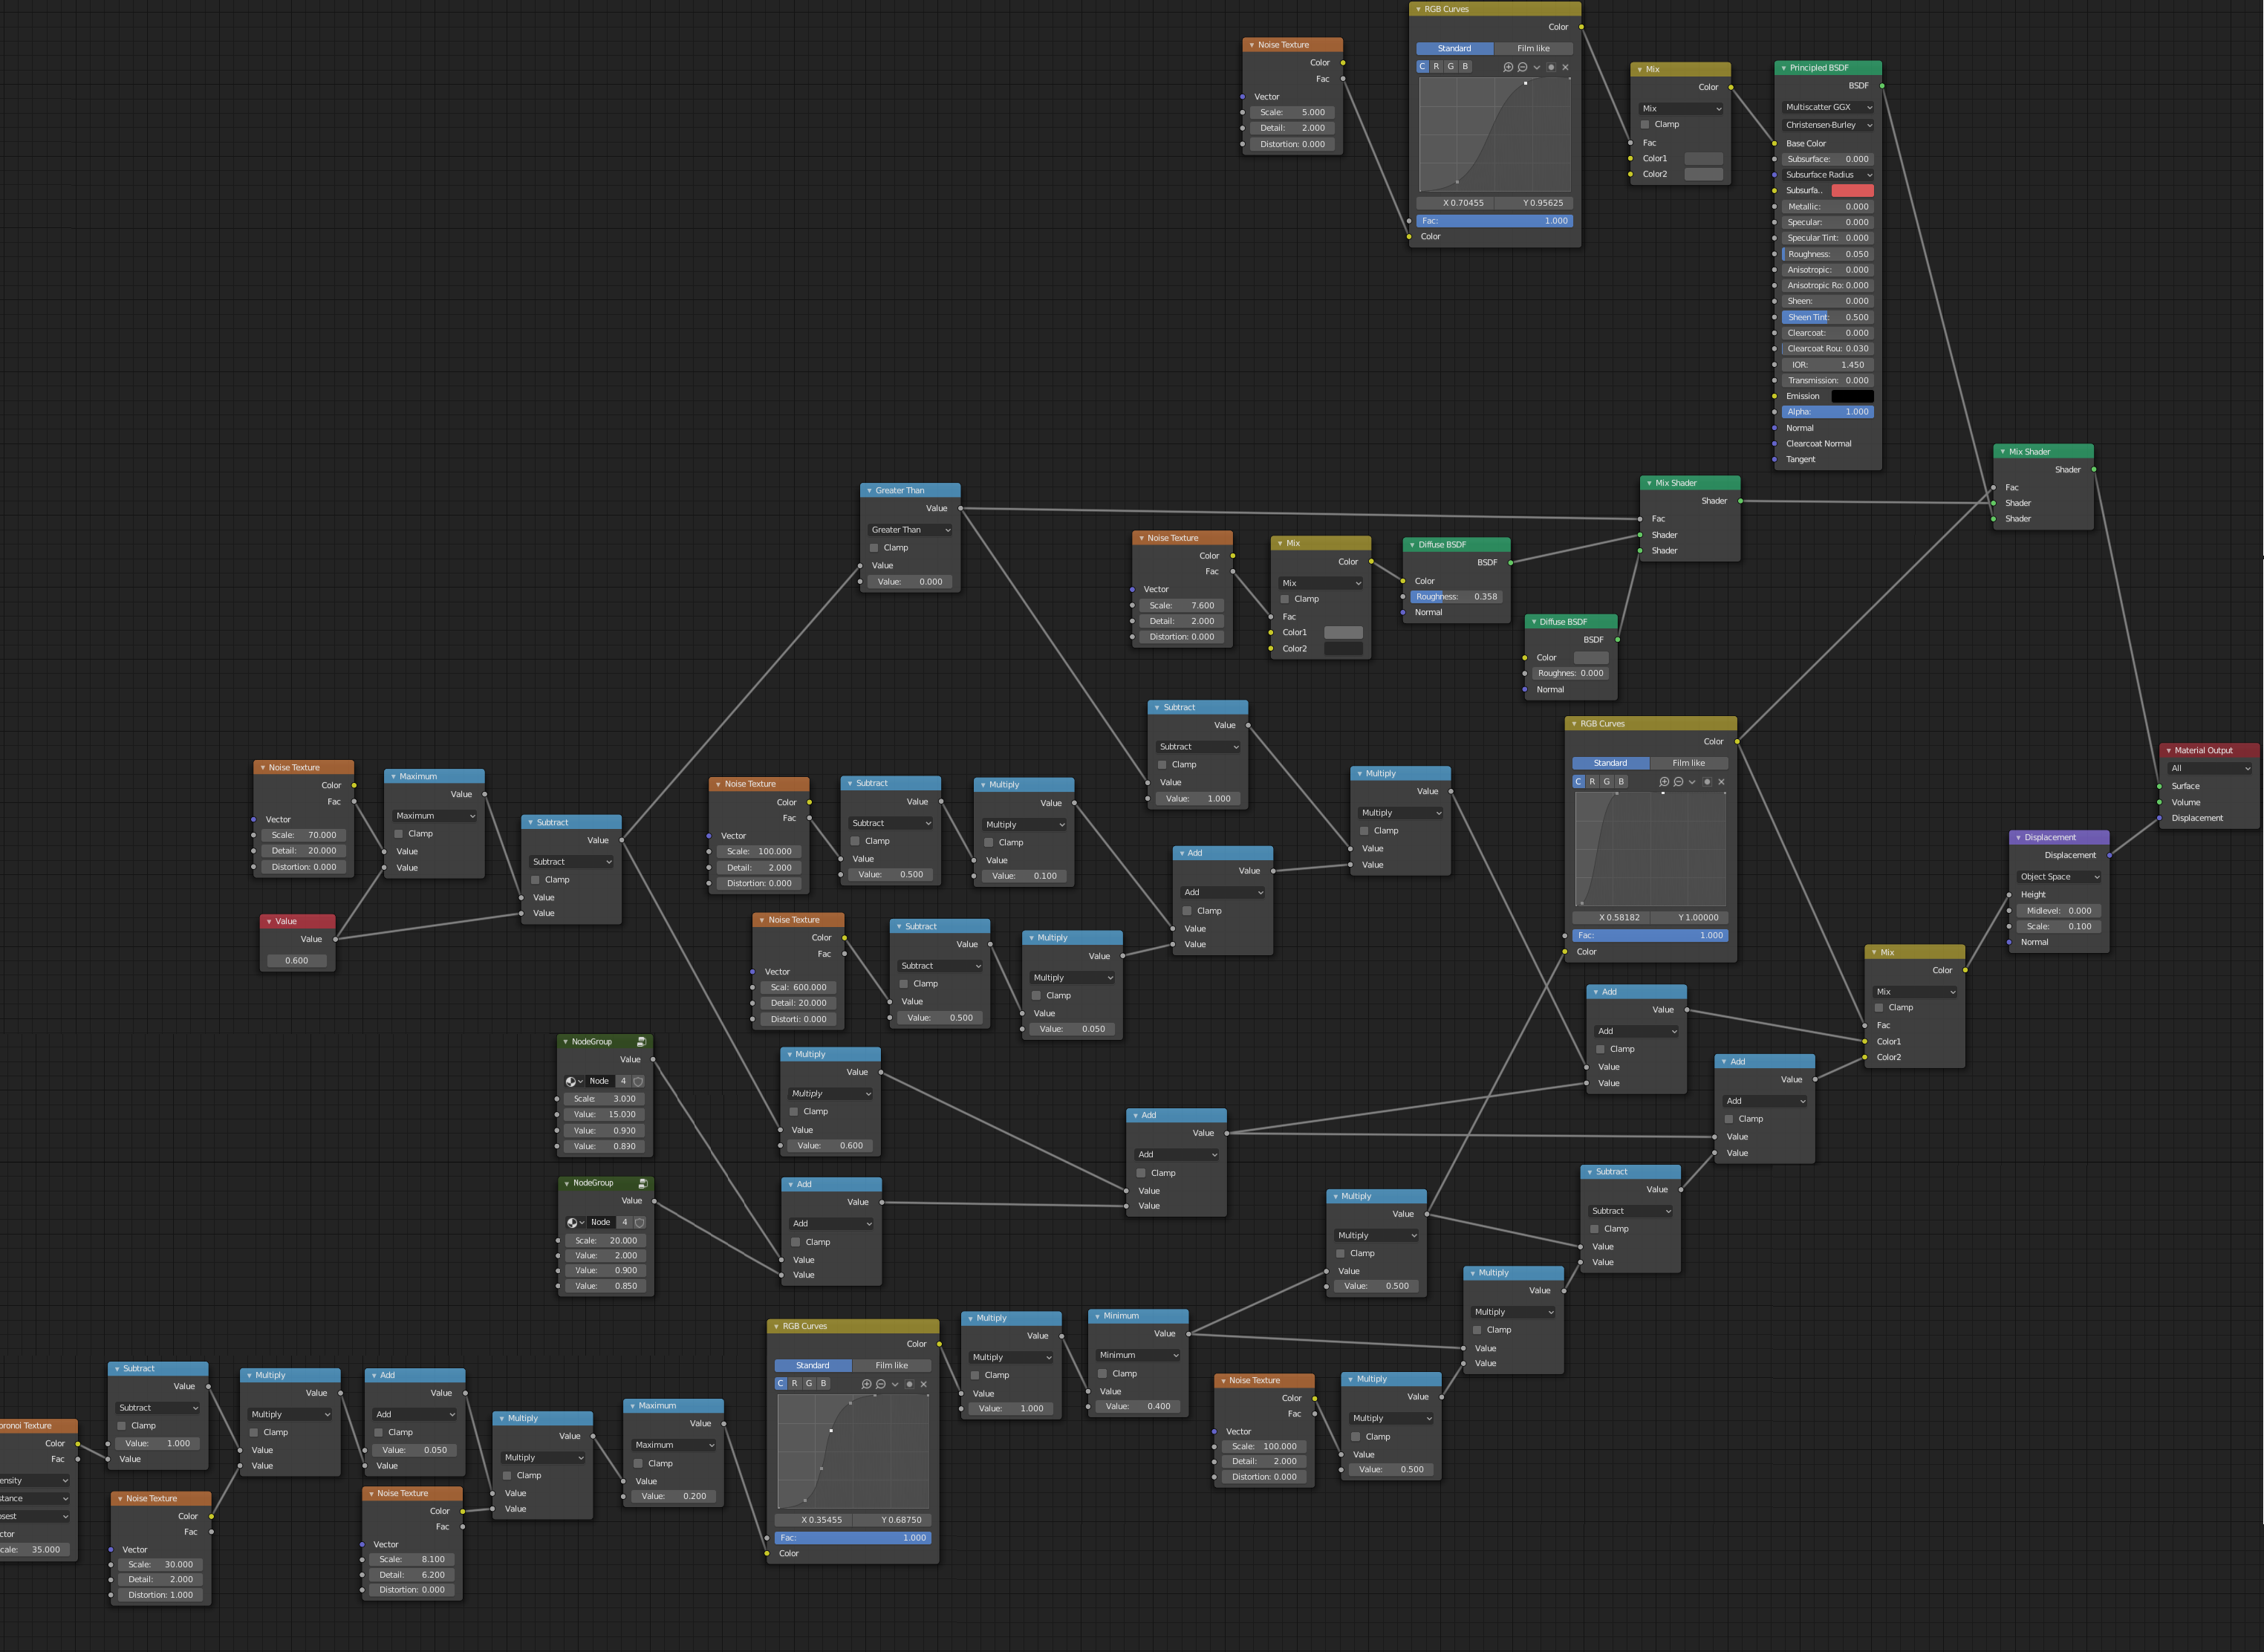
\includegraphics[height=.97\textwidth, angle=90]{doc/thesis/0_figures/procedural_terrain/node_network_highres.png}
    \caption{High resolution image of the shader node network used in \gls{sispo}.}
    \label{fig:node_highres}
\end{figure}


%\section{Toinen esimerkki liitteest\"a\label{LiiteB}}
%% Liitteiden kaavat, taulukot ja kuvat numeroidaan omana kokonaisuutenaan
%%
%% Equations, tables and figures have their own numbering in Appendices
%\renewcommand{\theequation}{B\arabic{equation}}
%\setcounter{equation}{0}  
%\renewcommand{\thefigure}{B\arabic{figure}}
%\setcounter{figure}{0}
%\renewcommand{\thetable}{B\arabic{table}}
%\setcounter{table}{0}

% Liitteiss\"a voi my\"os olla kuvia, jotka
% eiv\"at sovi leip\"atekstin joukkoon:
% %% Ymp\"arist\"on figure parametrit htb pakottavat
% %% kuvan t\"ah\"an, eik\"a LaTeX yrit\"a siirrell\"a niit\"a
% %% hyv\"aksi katsomaansa paikkaan. 
% %% Ymp\"arist\"o\"a center voi k\"aytt\"a\"a \centering-
% %% komennon sijaan
% %%
% %% Example of a figure, note the use of htb parameters which force
% %% the figure to be inserted here
% \begin{figure}[htb]
% \begin{center}
% 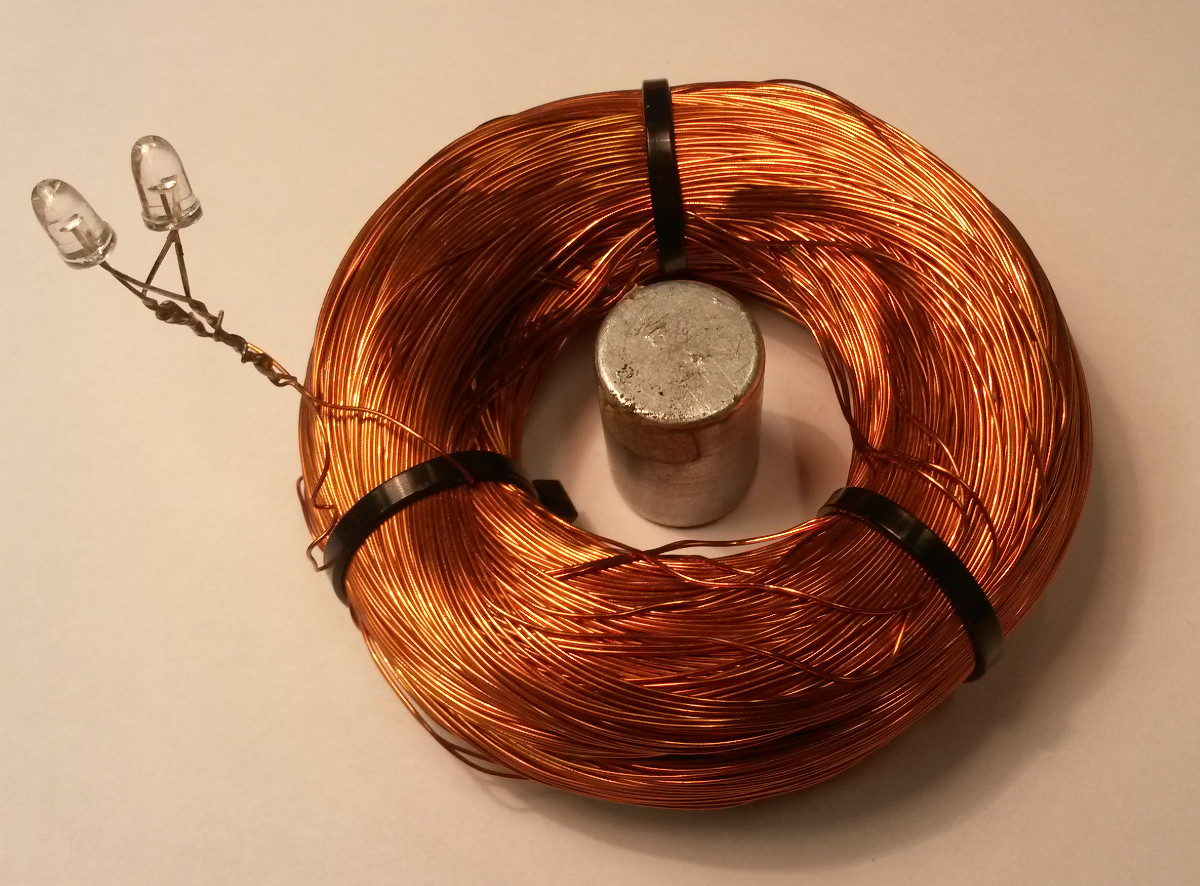
\includegraphics[height=8cm]{doc/thesis/0_figures/ledspole.jpg}
% \end{center}
% \caption{Kuvateksti, jossa on liitteen numerointi}
% \label{liitekuva}
% \end{figure}
% %%
% Liitteiden taulukoiden numerointi on kuvien ja kaavojen kaltainen:
% \begin{table}[htb]
% \caption{Taulukon kuvateksti.}
% \label{liitetaulukko}
% \begin{center}
% \fbox{
% \begin{tabular}{lp{0.5\linewidth}}
% 9.00--9.55  & K\"aytett\"avyystestauksen tiedotustilaisuus (osanottajat
% ovat saaneet s\"ahk\"opostitse valmistautumisteht\"av\"at, joten tiedotustilaisuus
% voidaan pit\"a\"a lyhyen\"a).\\
% 9.55--10.00 & Testausalueelle siirtyminen
% \end{tabular}}
% \end{center}
% \end{table}
% Kaavojen numerointi muodostaa liitteiss\"a oman kokonaisuutensa:
% \begin{align}
% T_{ik} &= -p g_{ik} + w u_i u_k + \tau_{ik},  \label{liitekaava3} \\
% n_i    &= n u_i + v_i.                      \label{liitekaava4}
% \end{align}